%iffalse
\let\negmedspace\undefined
\let\negthickspace\undefined
\documentclass[journal,12pt,onecolumn]{IEEEtran}
\usepackage{cite}
\usepackage{amsmath,amssymb,amsfonts,amsthm}
\usepackage{algorithmic}
\usepackage{graphicx}
\usepackage{textcomp}
\usepackage{xcolor}
\usepackage{txfonts}
\usepackage{listings}
\usepackage{enumitem}
\usepackage{mathtools}
\usepackage{gensymb}
\usepackage{comment}
\usepackage[breaklinks=true]{hyperref}
\usepackage{tkz-euclide} 
\usepackage{listings}
\usepackage{gvv}                                        
%\def\inputGnumericTable{}                                 
\usepackage[latin1]{inputenc}                                
\usepackage{color}                                            
\usepackage{array}                                            
\usepackage{longtable}                                       
\usepackage{calc}                                             
\usepackage{multirow}                                         
\usepackage{hhline}                                           
\usepackage{ifthen}                                           
\usepackage{lscape}
\usepackage{tabularx}
\usepackage{array}
\usepackage{float}
\usepackage{multicol}

\newtheorem{theorem}{Theorem}[section]
\newtheorem{problem}{Problem}
\newtheorem{proposition}{Proposition}[section]
\newtheorem{lemma}{Lemma}[section]
\newtheorem{corollary}[theorem]{Corollary}
\newtheorem{example}{Example}[section]
\newtheorem{definition}[problem]{Definition}
\newcommand{\BEQA}{\begin{eqnarray}}
\newcommand{\EEQA}{\end{eqnarray}}
\newcommand{\define}{\stackrel{\triangle}{=}}
\theoremstyle{remark}
\newtheorem{rem}{Remark}

\DeclareMathOperator{\taninv}{tan\,inverse}

% Marks the beginning of the document
\begin{document}
\bibliographystyle{IEEEtran}
\vspace{3cm}

\title{9.2.6 }
\author{S.Sai Akshitha - EE24BTECH11054}
\newpage
\maketitle
\bigskip

\renewcommand{\thefigure}{\theenumi}
\renewcommand{\thetable}{\theenumi}

\textbf{Question:} \\ Area of the region in the first quadrant enclosed by the $x$-axis, the line $y=x$ and the circle $x^2+y^2=32$ is \rule{1cm}{0.15mm}.  

\textbf{Solution:}
\begin{table}[ht!]    
  \centering
  \begin{tabular}[12pt]{ |c| c|}
    \hline
    \textbf{Variable} & \textbf{Description}\\ 
    \hline
    $P,Q$ & Points of intersection of line and circle \\
    \hline 
    $r$ & radius of the circle\\
    \hline
    $\theta$ & Angle between line $y=x$ and $x$-axis\\
    \hline
    $O$ & Centre of the circle(Origin)\\
    \hline 
    $A$ & Area of the portion \\
    \hline
    \end{tabular}

  
  \caption{Variables Used}
\end{table}

 Given line equation is 
 \begin{align}
    y=x
    \label{eq.1}
 \end{align} and circle equation is 
 \begin{align}
     x^2+y^2=32. \label{eq.2}
 \end{align} \\ By substituting \ref{eq.1} in \ref{eq.2}, we get \\ 
\begin{align*}
     \implies x^2+x^2&=32\\
 \implies 2x^2&=32\\
 \implies x^2&=16\\
 \implies x&=4,-4\\
\end{align*}
 
 After substituting the values of $x$ in \ref{eq.1}, we get the points of intersection as $P=\myvec{4,4}$ and $Q=\myvec{4,4}.$ 

Hence the area enclosed by the $x$-axis, the line $y = x$ and
the circle $x^2 + y^2 = 32$ is in the shape of a sector. \\ Area enclosed by the sector is given by 
\begin{align}
    A= \frac{1}{2}r^2\theta 
    \label{eq.3}
\end{align}
to find $r$, the distance between centre of circle and the point $P$ should be computed.\\
 \begin{align*}\norm{P}&=\sqrt{x^2+y^2} \\ &=\sqrt{4^2+4^2} \\ &=\sqrt{32} \\ &=4\sqrt{2}.\end{align*}\\
 To find the angle $\theta$, slope of the line is required, since the angle is between the given line and $x-$axis.\\ The line $y=x$ passes through the points $P$ and $Q$. Equation of line can be expressed as:\\
  \begin{align*} r = (1-t) \myvec{4,4}+ t
  \myvec{4,4}, t\in [0,1]\end{align*}\\
  Direction vector of $r$ is \\
   \begin{align*} d&= \myvec{4-(-4),4-(-4)} \\ &= \myvec{8,8} \\ &=\myvec{\Delta y , \Delta x }\end{align*} \\
   slope of the line=$\tan \theta = \frac{\Delta y}{\Delta x} =\frac{8}{8}=1.$\\
   \begin{align*}
       \implies \theta = \tan^{-1}(1)= \frac{\pi}{4}.
   \end{align*} \\Substituting the values in \ref{eq.3}, we get \begin{align*}
     A=4\pi.  
   \end{align*}


\begin{figure}[ht!]
   \centering
   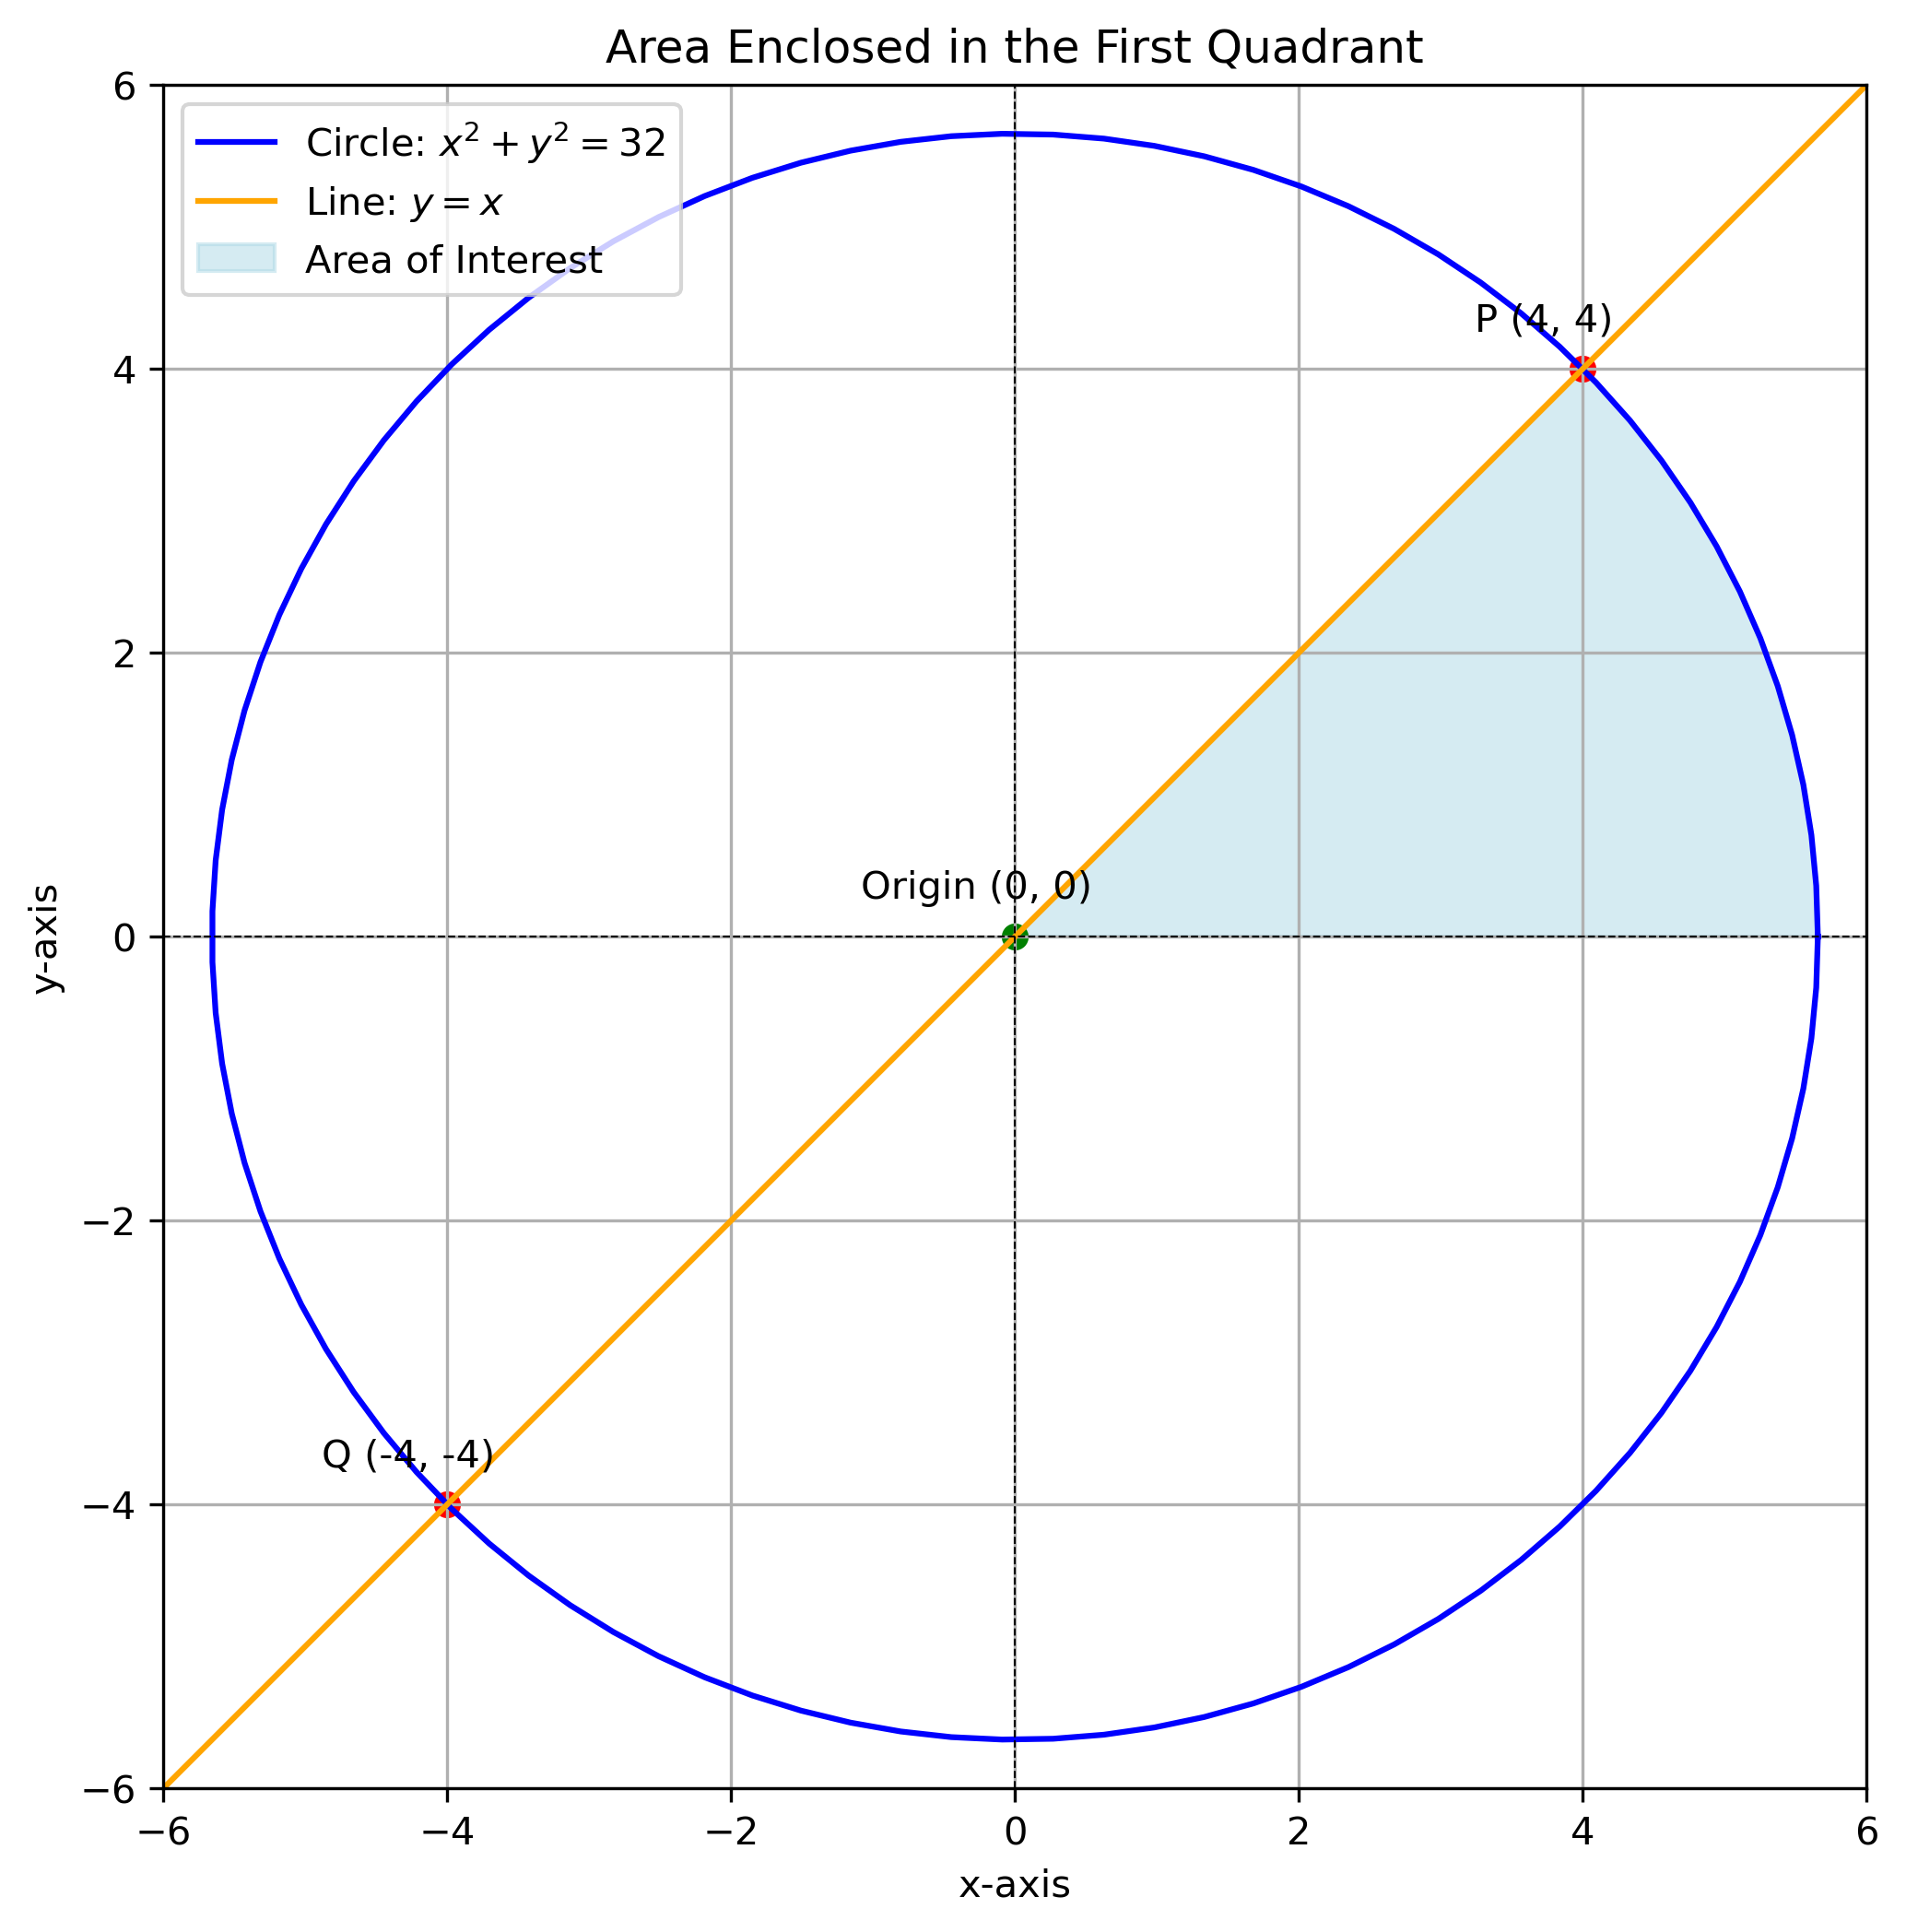
\includegraphics[width=0.7\linewidth]{circlenline.png}
    \label{stemplot}
\end{figure}


   
\end{document}
